%\subsubsection{Scalability}\label{size_physio_context}

We considered whether the model can scale to larger networks
by allowing the simulation to continue until the simulated network's size is equal to 
that of the corresponding BN, in contrast to previously described simulations (Figures \ref{adap_fig} and \ref{evol_figure}) which terminated when networks' size reached 
400 nodes. 
We performed four experiments in which the simulated networks were allowed to grow to a size
equal to that of Bacteria, Worm, Bacteria Regulatory, or Mouse Regulatory networks (see Table \ref{networks_summary} for their corresponding number of nodes/edges). 
The four experiments show the scalability of the model to larger networks, with the latter two further showing its scalability to 
the regulatory context (as opposed to all other networks which represent protein-protein interactions). 
Figure \ref{large_PPI}  shows the degree distribution of the 
the fittest network after multiple generations of mutate-and-select. The number of generations is approximately equal to that of the number
of nodes in the corresponding BN. In contrast to the smaller-sized evolved networks depicted in Figure \ref{evol_figure}, 
the larger simulation networks shown in Figure \ref{large_PPI} show an even smoother distribution particularly of hubs of degree $\geq$10. 
%\begin{comment}
\begin{figure*}[h]
		\centering
		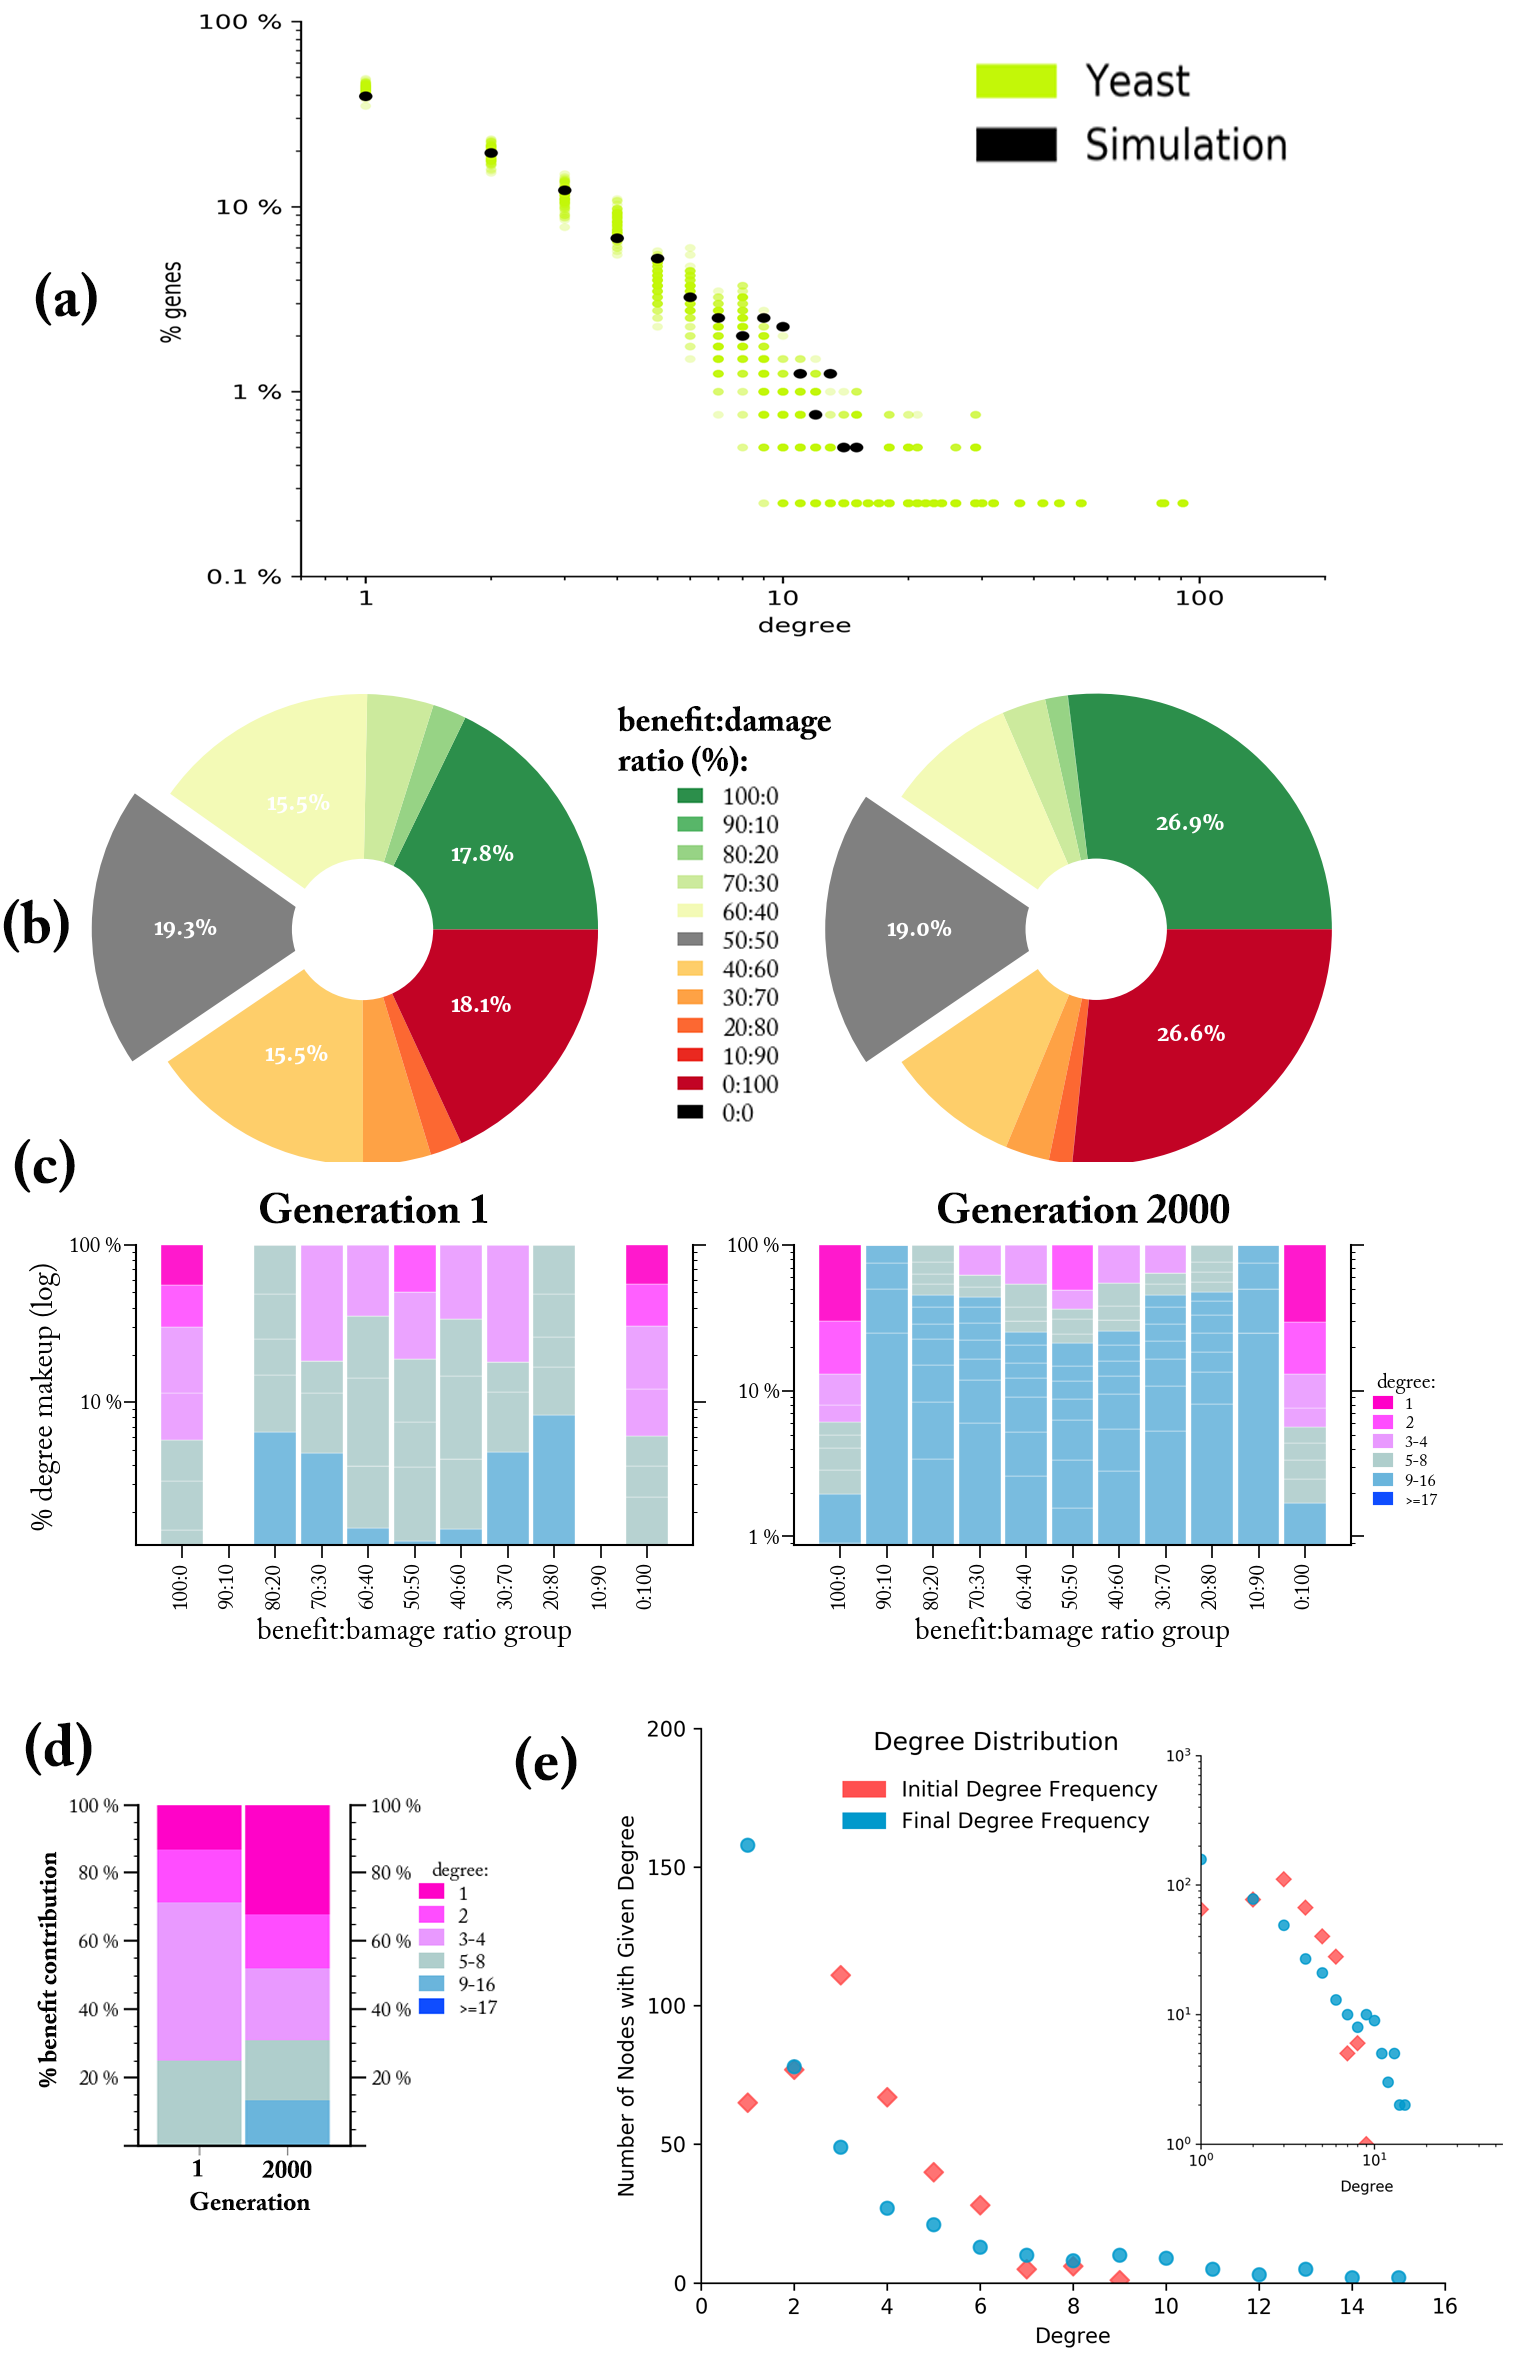
\includegraphics[width=17cm, height=10.5cm]{/results_additional/final/photoshop/processed.png}%origina ratio 1:0.77 width:height
		\caption{
				Scaling to larger networks and applicability to different physiological contexts. Networks start empty and undergo reassign-edge, add-node, 
				add-edge mutations. An evolving network grows by adding one node, and one or more edges while maintaining its edge:node ratio equal  
				that of its corresponding real BN. The simulation terminates when networks reach the same size (number of nodes) as that of the corresponding real BN. 
				The final 
				degree distribution of the fittest network is illustrated (horizontal black dashes) against that of the corresponding BN 
				(vertical coloured dashes). 
				Simulating against Bacteria and Mouse Regulatory networks (bottom row),  which are comprised of TF-gene, TF-TF and (in Mouse only) small RNA-gene 
				interactions as opposed to all 
				other networks which are comprised of protein-protein interactions, further shows the applicability of the model to different physiological contexts.
		}
		\label{large_PPI}
\end{figure*}	
%\end{comment}
	
		
		